\documentclass{article}
\usepackage[a4paper, margin=20mm]{geometry}
\usepackage{graphicx}
\usepackage{float}
\usepackage{subfigure}
\usepackage{amsmath}
\usepackage{amsfonts}
\title{Practical Submission Sheet}
\newcommand{\bb}[1]{\textbf{#1}}
\newcommand{\ol}[1]{\overline{#1}}
\date{}
\begin{document}
	\maketitle
	\begin{tabular}{ll}
		\bb{Term}: 2020-1 & \bb{Submission Date}: \today\\
		\bb{Lecture Date}: October 16, 2020. & \bb{Practical Number}: 8\\
		\bb{Course Code}: PHY249 & \bb{Section}: G2903\\
		\bb{Registration Number}: 11912610 & \bb{Roll No}: 03\\
		\bb{Student Name}: Aayush Arya & \\
	\end{tabular}
	
	\section*{Aim} To create XOR and NOT gates using NAND logic.

	\section*{Concepts Learnt}	
	
	
	\section*{Key Observations \& Insights}
	
	
	\section*{Application Areas}
	
	
	\section*{Report}
	
	\begin{figure}[H]
		\centering
		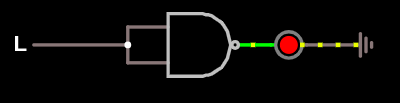
\includegraphics[width=0.75\textwidth]{NOT}
		\caption{NAND combination for constructing the NOT  (inverter) gate.}
		\label{circuit1}
	\end{figure}
	 
	 	\begin{table}[H]
	 	\centering
	 	\begin{tabular}{|c|c|}
	 		\hline
	 		Input & Output \\
	 		\hline 
	 		0 & 1\\
	 		1 & 0\\
	 		\hline
	 	\end{tabular}
	 	\caption{Truth table for the NAND combination. It can be seen that it behaves identically to a NOT gate.}
	 \end{table}
 
	


	\begin{figure}[H]
		\centering
		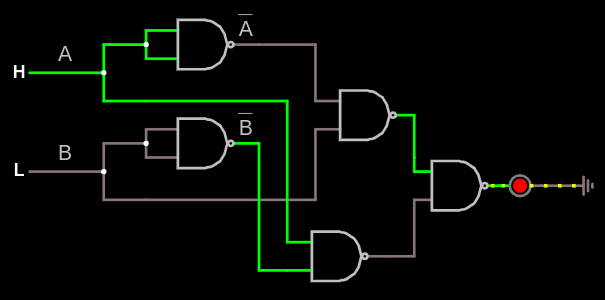
\includegraphics[width=0.75\textwidth]{XOR}
		\caption{NAND logic for the XOR gate.}
		\label{circuit2}
	\end{figure}

 
\begin{table}[H]
	\centering
	\begin{tabular}{|c|c|c|}
		\hline
		Input A & Input B & Output\\
		\hline
		0 & 0 & 0\\
		0 & 0 & 1\\
		0 & 1 & 1\\
		0 & 1 & 0\\
		\hline
	\end{tabular}
	\caption{Truth table for the logic system in Figure \ref{circuit2}}

\end{table}

	\begin{figure}[H]
		\centering
		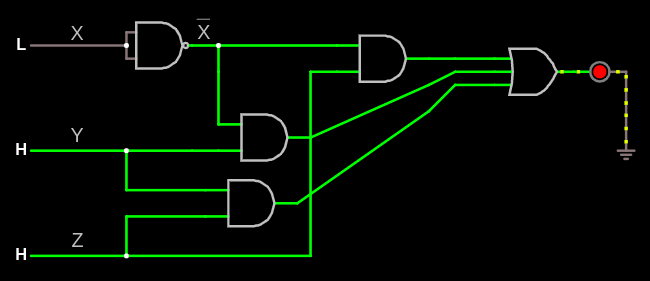
\includegraphics[width=0.85\textwidth]{extra}
		\caption{$f= \ol{X}.Y + \ol{X}.Z + Y.Z$}
		\label{}
	\end{figure}

\end{document}}